\documentclass{article}

% if you need to pass options to natbib, use, e.g.:
%     \PassOptionsToPackage{numbers, compress}{natbib}
% before loading neurips_2020

% ready for submission
% \usepackage{neurips_2020}

% to compile a preprint version, e.g., for submission to arXiv, add add the
% [preprint] option:
     \usepackage[preprint]{neurips_2020}

% to compile a camera-ready version, add the [final] option, e.g.:
%     \usepackage[final]{neurips_2020}

% to avoid loading the natbib package, add option nonatbib:
     %\usepackage[nonatbib]{neurips_2020}

\usepackage[utf8]{inputenc} % allow utf-8 input
\usepackage[T1]{fontenc}    % use 8-bit T1 fonts
\usepackage{hyperref}       % hyperlinks
\usepackage{url}            % simple URL typesetting
\usepackage{booktabs}       % professional-quality tables
\usepackage{amsfonts}       % blackboard math symbols
\usepackage{amsmath}
\usepackage{subfigure}
\usepackage{float}
\usepackage{multirow}
\usepackage{algorithm}
\usepackage{algorithmic}
\usepackage{graphicx}
\usepackage{nicefrac}       % compact symbols for 1/2, etc.
\usepackage{microtype}      % microtypography

\title{Formatting Instructions For NeurIPS 2020}

% The \author macro works with any number of authors. There are two commands
% used to separate the names and addresses of multiple authors: \And and \AND.
%
% Using \And between authors leaves it to LaTeX to determine where to break the
% lines. Using \AND forces a line break at that point. So, if LaTeX puts 3 of 4
% authors names on the first line, and the last on the second line, try using
% \AND instead of \And before the third author name.

\author{%
  Jiantao Qiu \\
  Department of Electronic Engineering\\
  Tsinghua University\\
  Haidian, Beijing, China\\
  \texttt{qjt15@mails.tsinghua.edu.cn} \\
  % examples of more authors
   \And
   Zhaoran Wang \\
   Industrial Engineering and Management Sciences\\
    Northwestern University\\
    Evanston, IL, USA\\
   \texttt{zhaoranwang@gmail.com} \\
   \AND
   Zhuoran Liu \\
   Industrial Engineering and Management Sciences\\
    Northwestern University\\
    Evanston, IL, USA\\
   \texttt{mailaddress@mailsever.com} \\
  \And
  Yu Wang \\
  Department of Electronic Engineering\\
  Tsinghua University\\
  Haidian, Beijing, China\\
  \texttt{yu-wang@mail.tsinghua.edu.cn} \\
  % \And
  % Coauthor \\
  % Affiliation \\
  % Address \\
  % \texttt{email} \\
  % \And
  % Coauthor \\
  % Affiliation \\
  % Address \\
  % \texttt{email} \\
}

\begin{document}

\maketitle

\begin{abstract}
The reinforcement learning algorithms work well with well-defined rewards, but fail with sparse/deceptive rewards and require additional exploration strategies. This work introduces a deep exploration method based on Upper Confidence Bound (UCB) bonus. The proposed method can be plugged-in the actor-critic algorithms that use deep neural networks as a critic. Based on the conclusion of the regret bound of under the Linear Markov Decision Process (MDP) approximation, we use the Feature Matrix to calculate the UCB bonus for deep exploration. The proposed method is equivalent to the count-based exploration method in special cases and is more suitable for general situations. Our method uses the last d-dimension feature vector in the critic network and is easy to deploy. We design a simple task ``Swim'' to demonstrate the principle of the proposed method to achieve exploration in sparse/deceptive reward environments. And we do more empirical evaluation on sparse/deceptive reward version gym environments. The evaluation results verify that the proposed algorithm can perform effective deep exploration in sparse/deceptive reward tasks.
\end{abstract}


\section{Introduction}
Reinforcement learning is a type of learning method that attempts to maximize the cumulative rewards an agent receives in the environment. In recent years, deep reinforcement learning algorithms using deep neural networks as function approximations have made impressive progress in solving continuous action control tasks, especially Actor-Critic algorithms such as TD3 \cite{TD3}, SAC \cite{SAC}, PPO \cite{PPO}, etc. These algorithms are widely used in tasks such as autonomous driving, drone flight, and robot control.

Reinforcement learning algorithms usually choose actions at each time step to maximize future cumulative reward based on the observed data; this is reflected in the optimal Bellman equation and the policy gradient. However, in more difficult tasks, the agent fails to improve the cumulative return or converge to the sub-optimal solution due to the lack of global data at the early stage of the training process, resulting in a non-efficient algorithm.

The most widely used exploration strategies in Actor-Critic algorithms are the indirectional exploration strategy, including $\epsilon$-greedy method \cite{DQN}, action-noise \cite{DDPG}, parameter-noise \cite{pnoise}, maximum entropy \cite{SQL}, etc. This type of method is easy to deploy but has no theoretical efficiency guarantee. The reason is that the indirectional method simply increases the probability of other non-optimal actions without specifying which states-actions need to be explored more. In principle, exploring states-actions with more uncertainty can explore the MDP more efficiently and make the algorithm converge to the global optimum.

Based on this principle, the Upper Confidence Bound (UCB) method \cite{auer2002finite,audibert2009exploration} and Thompson Sampling (TS) method \cite{TS,TStutorial} are proposed to design exploration strategies. The UCB method gives a higher additional bonus to state-actions with more uncertainty to explore these state-actions. The TS method samples value function from the posterior distribution based on the observed data and selects the optimal action so that the actions with more uncertainty are selected with a higher probability.

The UCB method and the TS method have been proved to be efficient in the case of tabular MDP \cite{TStutorial}, and have been implemented in Q-based algorithms on discrete action tasks \cite{BDQN,osband2018randomized}. However, the promotion of these exploration strategies in the Actor-critic algorithm on continuous action tasks is rare. Compared to Q-based algorithms, Actor-Critic algorithms are difficult to be compatible with TS directly. This is because TS algorithms usually sample on the posterior distribution, which results in the inconsistency of policy gradient estimated by sampled critics in each iteration step. According to this point, estimating the UCB and forming an exploration bonus is more suitable for Actor-Critic algorithm.

In recent works, the UCB method applied in the deep Actor-Critic algorithm mainly constructs a state density model $\rho(x)$ and induces the pseudocount and generates the exploration bonus by $N(s,a)^{-1/2}$ \cite{bellemare2016unifying,ostrovski2017count,machado2018count}. Among them, a state density estimation method is designed. The method of state density estimation is the core part of this kind of works. However, these works usually use heuristic design methods and lack theoretical efficiency guarantees. And it may be necessary to train additional network models, resulting in more computational overhead.

In this work, a method based on feature space pseudocount for forming the UCB bonus is proposed, which utilizes the ``$\phi(s,a)^\top w$'' structure of commonly used deep neural networks and references the theoretical analysis in Cai's work \cite{cai2019provably}. Our method can be plugged-in various state-of-the-art Actor-Critic algorithms. To demonstrate the performance of our method, a set of toy continuous action control task with different configurations are designed to verify that our algorithm. In addition, we modify the reward settings of several tasks in the gym \cite{gym} into sparse/deceptive reward versions and verify our method. The results show that the proposed algorithm can solve more complex sparse/deceptive reward tasks.

Here is an outline for the rest part of this article. In Section 2, the background relevant to this work is introduced. In Section 3, we cite the theoretical work of the regret bound and show how to implement Inverse-Cumulative-Feature Bonus to the Actor-Critic algorithms. In Section 4, we compare our method to the work most relevant to us. In Section 5, the results of empirical experiments on toy tasks and gym tasks are shown and explained. In the last section, we summarize this work and propose possible future work.

\section{Background}
\subsection{Notation}
We consider an MDP with discount factor and deterministic reward: $\langle \mathcal{S},\mathcal{A},\mathcal{P},r,\gamma \rangle$, where $\mathcal{S}$ is the state space and $\mathcal{A}\subset \mathbb{R}^{d_a}$ is the continuous action space, $\mathcal{P}(s'|s,a)$ is the transition probability, $r(s,a)$ is a deterministic reward function and $\gamma$ is the discount factor.

A typical Actor-Critic algorithm for continuous action tasks includes a Q-value approximation function $Q(s,a):\mathcal{S}\times\mathcal{A}\rightarrow\mathbb{R}$ and a policy function $\pi(a|s):\mathcal{S}\times\mathcal{A}\rightarrow\mathbb{R_+}$. In the context of the deep neural network they can be rewritten as $Q(s,a;\theta^{Q})$ and $\pi(a|s;\theta^{\pi})$. The commonly used Q-value neural network can be expressed as $Q(s,a;\theta^{Q}) = \phi(s,a;\theta^{\phi})^{\top}w$, in which $\phi(\cdot):\mathcal{S}\times\mathcal{A}\rightarrow\mathbb{R}^d$ is a non-linear mapping named "feature mapping" and $\phi^{\top}w$ is a linear mapping.

\subsection{Sparse and Deceptive Reward}
\label{sec:tasks}
Usually, a reward for a task is defined according to the needs of the application. For example, in the HalfCheetah task \cite{mujoco}, a half-body cheetah with 6 degrees of freedom is placed on the ground plane. In each time step, the reward is $r_t = r_{speed} + r_{control}$, where $r_{speed}$ is proportional to the distance to the right in this time step, and $r_{control} = -\alpha*||\vec{a_t}||^2_2$ is the action penalty. The implication behind the reward is that the agent is expected to achieve higher speed with minimal control cost. Since the agent is constrained to a two-dimensional vertical plane, any random action can cause the agent to move to the right and immediately get positive feedback. It is easy to sample a policy that can get a positive reward from policy space, and the positive reward will further drive the agent to learn how to run faster, thus forming positive feedback.

However, this well-defined situation does not always appear in all tasks, and positive feedback may not be easy to reach. In some tasks where the goal is to reach specific target states, a positive reward can only be obtained when the agent reaches these states. It means that the agent can only get 0 rewards before it happens to touch these states. The $Q(s,a)$ or $V(s)$ will learn to equal zero for any state and action, and make the policy gradient equal zero, the actor cannot be optimized anymore. In addition, in the control task, in order to reduce the energy consumed by controlling each joint, the action penalty term (as $r_{control}$ in HalfCheetah) will be included in the reward. Before getting any positive feedback, the agent will learn to keep the zero action as the best policy to minimize the penalty, and this further prevents the agent from making various exploratory actions. "Sparse reward" and "zero action" together led to the morass of exploration. In these cases, additional exploration strategies become especially important. Once the agent reaches the goal states and gains a positive reward through an additional exploration strategy, the critic will direct the actor to learn to access the goal states with a higher frequency and finally learn to solve the task.

\subsection{Exploration Strategy}
Among the current exploration strategies for model-free RL, indirectional exploration strategies are often used due to the convenience of deployment, including $\epsilon$ -greedy \cite{DQN}, action-noise \cite{DDPG}, parameter-noise \cite{pnoise}, maximum entropy methods \cite{SQL}, etc. This type of method has the problem of being inefficient for long horizon problems, in other words, it cannot achieve "deep exploration" \cite{osband2018randomized}. Achieving effective exploration requires following the "optimistic" principle: assigning higher visit probability to choices with more uncertainty. However, the indirectional method does not use the information of the past access status, and cannot correctly assign a higher probability to a choice with more uncertainty.

The TS method is a type of exploration algorithm that samples the posterior distribution of the value model and greedily chooses the optimal action based on the sampling results \cite{TStutorial}. Since the posterior sampling model replaces the maximum likelihood model, there is a higher probability of selecting a suboptimal action with large uncertainty. The key point of this type of work is how to sample the value model on the posterior distribution. Existing works include \cite{BDQN, osband2018randomized, lastLayerBayes}. However, for the Actor-Critic algorithms, the policy follows the critic by accumulating the policy gradient slowly, and is not able to reflect the results of the critical posterior sampling in time, which makes TS method difficult to be applied in Actor-Critic algorithms.

Different from the TS method, the UCB method uses the upper confidence bound of the posterior distribution of the value model to replace the maximum likelihood model and selects the action greedily to achieve exploration \cite{auer2002finite,audibert2009exploration}. A standard method of this type of method is to give an estimate of the uncertainty of the value model as a bonus added to the original reward of the task. Since the bonus changes slowly with the number of training rounds, the effect on actors during a training session is consistent. Compared with TS method, UCB method is more compatible with Actor-Critic method.
\section{Exploration by UCB bonus}
We cite Cai's \cite{cai2019provably} theoretical work on regret decomposition and the upper bound of model prediction error under linear MDP approximation. Then we introduce the Actor-Critic algorithm with UCB bonus in the context of deep neural networks.

\subsection{Regret Decomposition}
In \cite{cai2019provably} paper, an Optimistic Policy Optimization (OPPO) algorithm is proposed for the MDP with adversarial rewards and stochastic transition dynamics. The policy improvement step and the policy evaluation step can be briefly expressed as:
\begin{eqnarray}
    &&\pi_h^{k+1}(\cdot,\cdot)\propto \pi_h^k(\cdot,\cdot)\cdot \text{exp}\{\alpha\cdot Q_h^k(\cdot,\cdot)\}\\
    &&Q_h^k(\cdot,\cdot)\leftarrow r_h^k(\cdot,\cdot)+\mathbb{E}_{\hat{\mathbb{P}}(s'|\cdot,\cdot)}[V^k_{h+1}(s')]\\
    &&V^k_h(\cdot)\leftarrow \langle Q_h^k(\cdot,\cdot),\pi^k_h(\cdot,\cdot)\rangle
\end{eqnarray}


The regret of the OPPO algorithm can be de down into three terms:
\begin{equation}
    \begin{split}
        &\text{Regret}(T)=\sum_{k=1}^K(V_1^{\pi^*,k}(s^k_1)-V_1^{\pi^k,k}(s^k_1))\\
        &=\underbrace{\sum_{k=1}^K\sum_{h=1}^H\mathbb{E}_{\pi^*}[\langle Q^k_h(s_h,\cdot),\pi^*_h(\cdot|s_h)-\pi^k_h(\cdot|s_h) \rangle|s_1=s_1^k]}_{(i)}\\
        &+\underbrace{\mathcal{M}_{K,H,2}}_{(ii)}\\
        &+\underbrace{\sum_{k=1}^K\sum_{h=1}^H(\mathbb{E}_{\pi^*}[\iota_h^k(s_h,a_h)|s_1=s_1^k]-\iota_h^k(s_h^k,a_h^k))}_{(iii)}
    \end{split}\label{eq:regret}
\end{equation}

The term (i) is due to the adversarial reward. Since in each turn the reward function is selected by the adversary, the policy improvement step size needs to be selected carefully to avoid being too "extreme" or too "conservative". The term (ii) is a martingale which is associated with the stochastic transition dynamics.

We focus on the third item, where $\iota$ is the \textbf{model prediction error} which defined as:
\begin{equation}
\iota_h^k(s,a) = r_h^k(s,a) + \mathbb{E}_{\mathbb{P}_h(s'|s,a)}[V_{h+1}^k(s')] -Q_h^k(s,a)
\end{equation}
This term is because only limited historical data is used to update $Q$ by Bellman Equation, which results in the predict $Q$ differs from $r+\mathbb{E}_{\mathbb{P}(s'|s,a)}[V(s')]$ with real transition dynamics  $\mathbb{P}(s'|s,a)$. To bound the third term we need more assumptions on the property of MDP.

\subsection{Linear MDP Approximation}
To further analyze the bounds of the third term, the linear MDP approximation is introduced. We assume that the MDP is a linear MDP with feature mapping $\phi : \mathcal{S}\times \mathcal{A} \rightarrow \mathbb{R}^d$. That is there exist $d$ measures $\mu_h=(\mu_h^1,\cdots,\mu_h^d)\top$ on $\mathcal{S}$ and a vector $\theta_h^k \in \mathbb{R}^d$ such that:
\begin{align}
    \mathbb{P}_h(s'|s,a)&=\phi(s,a)^\top\mu_h(s')\\
    r_h^k(s,a)&=\phi(s,a)^\top\theta^k_h
\end{align}
Under the linear approximation, there exist vector $w_h^{\pi,k}\in\mathbb{R}^d$ for any policy $\pi$ such that:
\[Q_h^{\pi,k}(s,a) = r_h^k(s,a)+\phi(s,a)^\top w_h^{\pi,k}\]
The $w_h^{\pi,k}$ can be estimated by Least-Squares Temporal Difference (LSTD) method:

\begin{align}
    & \Lambda_h^k \leftarrow \sum_{k=1}^{K}\phi(s_h^k,a_h^k)\phi(s_h^k,a_h^k)^\top+\lambda\cdot I\\
    & w_h^k \leftarrow (\Lambda_h^k)^{-1}\sum_{k=1}^{K}\phi(s_h^k,a_h^k) V^k_{h+1}(s_{h+1}^k)\\
    & Q_h^k(s,a)\leftarrow r_h^k(s,a) + \phi(s,a)^\top w_h^k \label{eq:LSTD}
\end{align}
    
By add bonus $\beta[\phi(s,a)^\top(\Lambda_h^k)^{-1}\phi(s,a)]^{1/2}$ on right-side of Equation (\ref{eq:LSTD}) and select 
\[\beta=CdH\sqrt{\log(dT/\zeta)}\]
the regret term (iii)  in Equation (\ref{eq:regret}) is bounded by 
\[\text{Regret}(T) \leq 2C\sqrt{2d^3H^3T}\log(dT/\zeta)\]
with probability at least $1-\zeta/2$.

\subsection{Optimistic Actor-Critic}
So far we have introduced the results of Cai's article on the regret bound under the linear MDP approximation. To achieve a practical exploration strategy, we consider the context of function approximation via deep neural network and proposed \textbf{LI}near \textbf{F}eature \textbf{E}xploration Bonus (LIFE).

We take Actor-Critic algorithms represented by DDPG, TD3, and SAC as examples. This type of algorithm usually maintains a critic network $Q(s,a;\theta^Q)$ and an actor network $\pi(a|s;\theta^\pi)$. The critic network minimizes the mean square error of the output and bootstrap target: \[L^Q=\mathbb{E}[(Q(s,a)-Q^{target}(s,a))^2]\]
The bootstrap target is :
\[Q^{target}(s,a)=r(s,a)+\gamma Q^-(s',a')\]
where $Q^-$ is the target critic, and $a'$ is sampled by the target actor $\pi^-(a|s')$. The actor network is updated by policy gradient:
\[\nabla J=\mathbb{E}[Q(s,a)\cdot \nabla\log(\pi(a|s))]\]
or by reparameterization trick: 
\[\nabla J=\mathbb{E}[\nabla_a Q(s,a)|_{a=\mu} \cdot \nabla \mu(s,\epsilon)]\]
where $\mu(s,\epsilon) \sim \pi(a|s)$ where $\epsilon$ is a random variable following some known distribution such as gaussian distribution.

Fig \ref{fig:critic} shows the structure of a typical critical network. State-action data is input to the critic network and a feature vector $\phi(s,a) \in \mathbb{R}^d$ is output through non-linear mapping, then pass to a linear layer $\phi^{\top} w$ to output the Q value $Q(s,a)$. We use $\phi(s,a)$ as the feature in the linear-MDP approximation for calculate LiFE bonus

\begin{figure}[!htb]
    \centering
    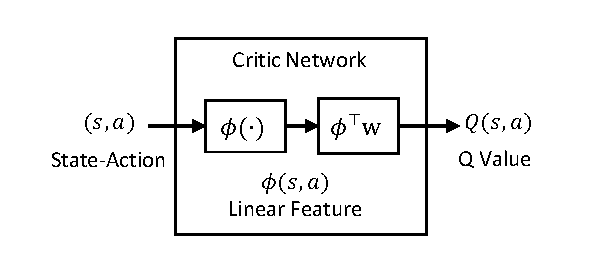
\includegraphics[width=230pt]{figs/Critic.pdf}
    \caption{Structure of a critic network contains a non-linear feature layer $\phi(\cdot)$ and a linear layer $\phi^{\top}w$.  }
    \label{fig:critic}
\end{figure}

\begin{algorithm}[!htb]
    \caption{Linear Feature Exploration Bonus}
    \label{alg:DE-AC}
    \begin{algorithmic}
        \STATE {\bfseries Input:} MDP $\mathcal{M} = <\mathcal{S},\mathcal{A},\mathcal{P},r,\gamma>$,
        \STATE Initialize critic $Q(s,a;\theta^Q)$ , actor $\pi(a|s;\theta^\pi)$
        \STATE Initialize replay buffer $D = \emptyset$, and temp buffer $T = \emptyset$.
        \STATE Initialize target network $Q^-= Q$, $\pi^-= \pi$.
        \STATE Initialize Feature Matrix $\Lambda = \lambda I$.
        \FOR{1 {\bfseries to} step\_number}
        \STATE Take action by $a \sim \pi(a|s;\theta^\pi)$
        \STATE Rollout data $s' \sim \mathcal{P}(s'|s,a)$,$r = r(s,a)$
        \STATE $T \leftarrow T\cup {<s,a>}$,$D \leftarrow D\cup {<s,a,r,s'>}$
        \IF  {$|T|=N_{temp}$}
        \STATE $\Phi \leftarrow [\phi(s_1,a_1),\phi(s_2,a_2),\cdots ]$ for each $s_i\in T$
        \STATE $\Lambda \leftarrow \Lambda + \Phi \Phi^\top $
        \ENDIF 
        \STATE Sample data batch $\{d=(s,a,r,s')\}$ from $D$
        \STATE $\Gamma = \beta [\phi(s,a)^\top(\Lambda)^{-1}\phi(s,a)]^{1/2}$
        \STATE $a'\sim \pi^-(a|s')$, $target  = r + \Gamma + Q^-(s',a')$
        \STATE $L^Q=\sum(Q(s,a)- target)^2$
        \STATE $\theta^Q \leftarrow \theta^Q - \alpha^Q\cdot\nabla_{\theta^Q} L^Q$
        \STATE $L^\pi=-\sum [\nabla\log(\pi(a|s)) \cdot Q(s,a)]$
        \STATE $\theta^\pi \leftarrow \theta^\pi -\alpha^\pi\cdot\nabla_{\theta^\pi} L^\pi$
        \STATE Soft update target network $Q'$ and $\pi'$
        \ENDFOR
     \end{algorithmic}
     \end{algorithm}

The calculation of LiFE bonus involves the operation of matrix inversion, which is numerically unstable. To solve this problem, we convert the data type from float32 to float64 when performing calculations related to the Feature Matrix. In addition, considering that the Feature Matrix $\Lambda$ is a symmetric matrix, we use symmetric eigenvalue decomposition $\Lambda = Q E Q^\top+\lambda I$ to make the calculations stable as follow:
\begin{equation}
    \begin{aligned}
    \phi^\top (\Lambda)^{-1}\phi &= \phi^\top (QEQ^\top+\lambda I)^{-1}\phi\\
    &= \phi^\top (Q(E+\lambda I)Q^\top)^{-1}\phi\\
    &= (Q^\top\phi)^\top (E+\lambda I)^{-1}(Q^\top\phi)
    \end{aligned}
\end{equation}

During the training process, the feature mapping part of the critical network is constantly changing. But recalculating the feature vector corresponding to all the data in the replay buffer and updating $\Lambda$ will cause too much overhead. As an approximation, we store the new transition data into a temporary buffet $T$ and update 
\[\Lambda \leftarrow \Lambda+ \sum \phi(T)\phi(T)^\top\]
 every $N_{temp}$ steps. The pseudo code of the entire algorithm is shown as Alg. \ref{alg:DE-AC} .


\section{Related Work}
In this rection we introduce and compare some of the work most relevant to our method.

In \cite{lastLayerBayes}, the author uses the linear feature $\Lambda = \sum \phi\phi^\top+\lambda I$ to estimate the uncertainty of the Q-value estimate. They use the TS method, constructe covariance matrix $Conv=(\Lambda)^{-1}$ of the last layer w, then sampling on the distribution of $w\sim\mathcal{N}(\bar{w},Conv)$ and greedily adopting the largest action by  $a = \arg\max_{a\in\mathcal{A}}\phi(s,a)^\top w$. The same single-step bonus is derived, if converte the variance of the Gaussian distribution into UCB bonus $\beta[\phi^{\top}(\Lambda)^{-1}\phi]^{1/2}$ which is equivalent to this paper's work. The difference is that method proposed in \cite{lastLayerBayes} does not accumulate uncertainty through $H$. The effect of uncertainty only apply on one single step and is not passed through $\langle s, a, s' \rangle $. This means that the uncertainty in future steps cannot influence the decision of the current step, so that deep exploration cannot be achieved. This is reflected in his analysis of the regret world. In the case of $ H = 1 $, $ \text{Regret} (T) <C \sqrt {d ^ 2T} \log (T) $. But in the case of $ H> 1 $, the upper bound contains a $ \sqrt{\rho^H_\lambda} $ factor, which increases rapidly with the increase of H. This indicates that only by accumulating uncertainty can achieve right exploration.

In \cite{UBE} 's work, the same linear feature is also used to estimate the uncertainty of Q-value estimation and the TS method is applied as the exploration strategy. In their work, the uncertainty of the single-step Q estimation is accumulated by $ u^{target} = \phi ^ {\top} (\Lambda) ^ {-1} \phi + \gamma ^ 2 u (s ', a') $  which called Uncertainty Bellman 
Equation (UBE), which can be compared to an MDP with reward of $ \phi ^ {\top} (\Lambda) ^ {-1} \phi $, and a discount factor of $ \gamma ^ 2 $. The method proposed by \cite{UBE} is very close to ours, but apart from the differences in TS and UCB methods, the motivation is also different in source of uncertainty. Their method considers the uncertainty of the reward function and the transition function and uses the condition-independent property to derive the squared cumulative UBE, which is related to \textbf{Aleatoric Uncertainty}. Our method considers the error generated by fitting the MDP in the $\mathcal{R}^d$ space using the least squares method for finite number of observation samples, which is related to \textbf{Epistemic Uncertainty}. Due to the lack of analysis of the regret bound of the method proposed by \cite{UBE}, need more research to distinguish the difference between the two methods.

Our method is also related to the count-based method. Considering a tabular MDP with $ | {(s_i, a_i)} | = d $ where $(s_i,a_i)$ is the i-th state-action pair, we can set $ \phi (s_i, a_i) = [\phi_1, \phi_2, \cdots, \phi_d]^\top $ where $ \phi_j = \delta (i, j) $. We have 
\begin{eqnarray}
    && r(s_i, a_i) = \phi (s_i, a_i) ^ \top \theta\\
    && P(s_j | s_i, a_i) = \phi (s_i, a_i) ^ \top \mu (s_j) 
\end{eqnarray} 
 where $ \theta_i = r(s_i,a_i)$ and  where $ \mu (s_j)_i = P (s_j | s_i, a_i)$. Under these settings we have
 \begin{align}
 \Lambda &= \sum \phi \phi ^ \top + \lambda I \\
 &=diag (n_1 + \lambda, n_2 + \lambda, \cdots , n_n + \lambda)
 \end{align}
and 
 \[ \beta [\phi (s_i, a_i) ^ \top (\Lambda) ^ {-1} \phi (s_i, a_i)] ^ {1/2} = \frac{\beta} {\sqrt{n_i + \lambda}} \]
 which is equivalent to constructing a Model-Based Interval Estimation with Exploration Bonus (MBIE-EB) \cite{strehl2008analysis} using the exact count with $\lambda$ Laplacian smoothing. This example provides clues to the link between LiFE bonus and count-based bonus.

 There are some works based on count-based bonus construct density estimates $ \rho (s) $ and generate pseudocount based on 
 \[N (s) = \frac{\rho(s)(1-\rho'(s))}{\rho'(s)-\rho(s)}\]
 such as feature density model \cite{martin2017count}, neural density model \cite{ostrovski2017count}, successor representation \cite{machado2018count}, etc. The method in \cite{martin2017count} is the closest to our work , they consider that all the dimensions in the feature are independent other and constructs a density estimate by $\prod_{i=1}^d\rho_i(\phi_i(s))$, which is different from our linear feature approximation. These methods lack the guarantee of theoretical regret bounds, and may need to train additional neural networks and cause more computational overhead.
\section{Empirical Experiment}

In this section, we will first introduce a task with a low-dimensional continuous state-action space. This task can have different exploration difficulties by changing parameter configurations. Experiments on this task prove that our algorithm can achieve deep exploration. Then we modify the reward settings of the tasks on the Gym environment to be sparse or deceptive rewards. The results of these tasks show that our algorithm can solve more complex sparse reward tasks.

In the following experiments, we use the SAC algorithm with a double critical network and an automatic temperature adjustment as the baseline. By using the input of the last fully connected layer of one of the critics as the feature vector for calculating the Feature Matrix $\Lambda$, and selecting $ \beta = 10 $ as the coefficient of the UCB bonus. 

\begin{table*}[!htb]
    \centering
    \begin{tabular}{ccrrrrrrrrr}
    \toprule
    \multirow{2}{*}{$\Delta$} & \multirow{2}{*}{$1/\Delta$} &  & \multicolumn{2}{c}{well-defined task} &  & \multicolumn{2}{c}{sparse task} &  & \multicolumn{2}{c}{deceptive task} \\ \cline{4-5} \cline{7-8} \cline{10-11} 
                       &                      &  & $\beta=0.0$          & $\beta=10.0$         &  & $\beta=0.0$                 & $\beta=10.0$  &  & $\beta=0.0$           & $\beta=10.0$           \\ \hline
    0.0800             & 12.50                &  & 600            & 2200           &  & 1800                  & 3200    &  & 4100            & 3200             \\
    0.0700             & 14.29                &  & 700            & 2900           &  & 2800                  & 3600    &  & $>20000$           & 3600             \\
    0.0600             & 16.67                &  & 1200           & 3200           &  & 5100                  & 5000    &  & $>20000$           & 4500             \\
    0.0514             & 19.46                &  & 1300           & 3500           &  & 16600                 & 6100    &  & $>20000$           & 5200             \\
    0.0450             & 22.22                &  & 1700           & 3900           &  & $>20000$   & 8300    &  & $>20000$           & 7200             \\
    0.0400             & 25.00                &  & 2000           & 4600           &  & $>20000$   & 10800   &  & $>20000$           & 10600            \\
    0.0360             & 27.78                &  & 2400           & 5500           &  & $>20000$   & 11400   &  & $>20000$           & 13600            \\
    0.0327             & 30.56                &  & 2500           & 5100           &  & $>20000$   & 12700   &  & $>20000$           & 15200            \\ \bottomrule
    \end{tabular}
    \caption{Sample number need for solving different step coefficient $\Delta$ in well-defined, sparse and deceptive reward tasks }
    \label{tab:sample-number}
    \end{table*}

\subsection{Continuous Action Swim Task}
In order to measure the exploration ability of the proposed algorithm, we design a ``Swim'' task. This task has state space $ \mathcal{S} = [0,1]$, action space $ \mathcal{A} = [-1,1] $. Its state transfer function and reward function can be expressed by the following formula:

\begin{eqnarray}
    f(s) &=& -A \sin(2\pi \omega \cdot s) \\
    e(s,a) &=& \cos(\pi\cdot (a-f(s)))\\
    s'(s,a) &=& clip(s + \Delta \cdot e(s,a),0,1)\\
    r(s,a) &=& r_s\cdot s^l + r_a \cdot e(s,a)
\end{eqnarray}

\begin{figure}[!htb]
\centering
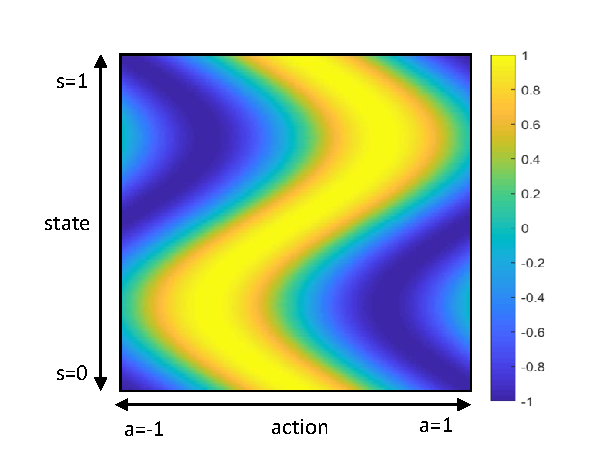
\includegraphics[width=230pt]{figs/Swim.pdf}
\caption{Effect $e(s,a)$ with $f(s) = -0.5\times \sin(2\pi\cdot s)$ in task Swim }
\label{fig:swim}
\end{figure}

Where $e(s,a)\in [-1,1] $ represents the effect of action $a$ in the state $s$, it reaches the maximum value $+1$ when $a=f(s)$ and reaches the minimum value $-1$ when $a= f(s)\pm 1 $. The effect affects both the state transition and the reward function. At each step, the state moves forward by $ \Delta \cdot e(s,a) $ and is truncated to the interval of $ [0,1] $. The task always starts at $ s_0 = 0 $ and resets after $ H = 100 $ steps. Each step of the reward includes two parts: the state reward $ r_s \cdot s ^ l $ and the action reward $ r_a \cdot e (s, a) $. The state reward is designed as a power function of $ s $ exponent $ l >> 1 $, so that the state reward is approximately distributed in the area of $ [1-1/l, 1] $. The action reward is designed to be proportional to the effect $ e(s, a) $ of the current action $ a $. When $ r_a> 0 $, it will guide the strategy forward, when $ r_a <0 $, it will guide the strategy back, and $ r_a = 0 $ has no guiding effect. These three cases correspond to "well defined", "deceptive", and "sparse", respectively.

\begin{figure}[!htb]
    \centering
       \subfigure[Sparse swim task with $\beta=10$]{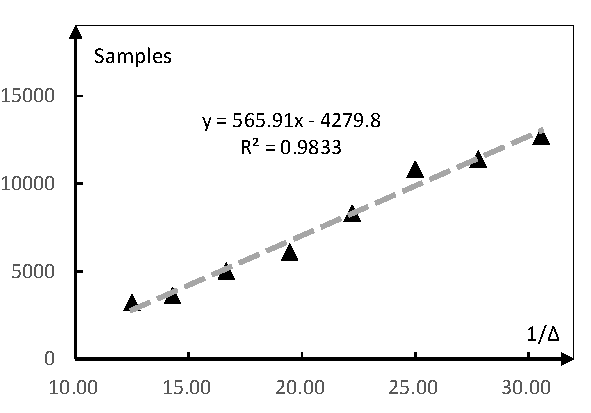
\includegraphics[width=180pt]{figs/Sparse.pdf}}
       \subfigure[Deceptive swim task with  $\beta=10$]{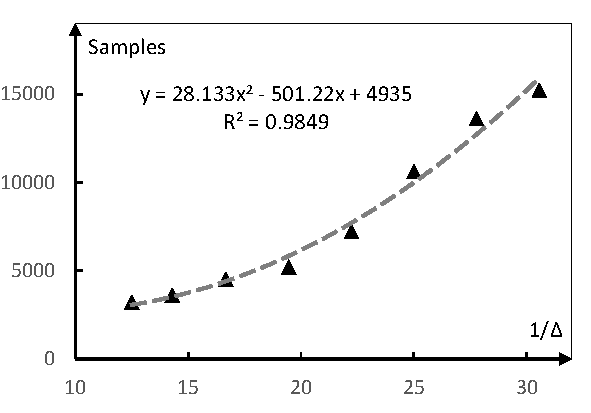
\includegraphics[width=180pt]{figs/Deceptive.pdf}}
    \caption{Scatter plot of $1/\Delta$-samples for sparse reward (top) and deceptive reward (down).}
   \label{fig:H-sample} 
\end{figure}
We perform experiments on different $ \Delta $ under the above three reward configurations. Each experiment is repeated ten times. We used the median curve to reach half of the reward when solving the task for the first time as the solving time of the task, and calculated the number of samples required to solve the task in each experiment as shown in the Table \ref{tab:sample-number}. The $>20000$ means the agent fail to reach state $s=1$ in $20000$ samples.

\begin{figure}[!htb]
    \centering
       \subfigure[Task with different $A$]{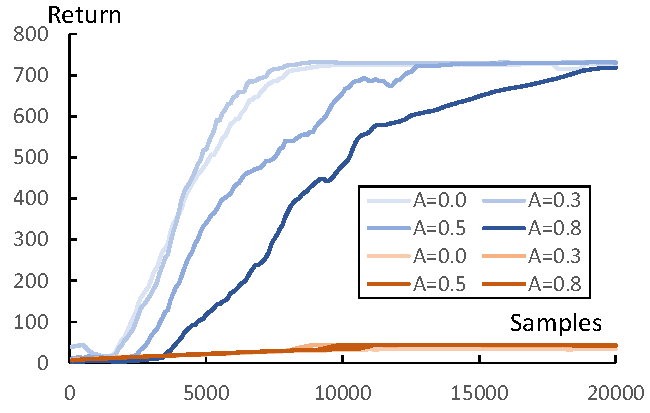
\includegraphics[width=180pt]{figs/A.pdf}}
       \subfigure[Task with different $\omega$]{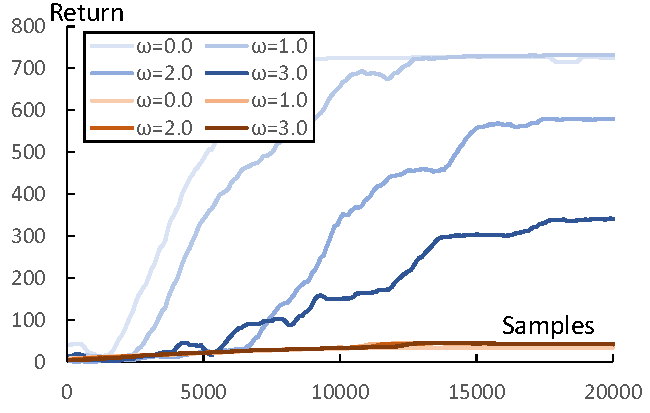
\includegraphics[width=180pt]{figs/f.pdf}}
    \caption{Mean return curve for different task configurations. The blue curve is $\beta = 10.0$ and the red is $\beta = 0.0$}
   \label{fig:A-f} 
\end{figure}

For a more intuitive understanding, we will plot the results on the sparse and deceptive tasks on the "$1/\Delta$-samples" axis in Fig \ref{fig:H-sample}. On sparse rewards, the sample required by our method to solve the task increases linearly with H, but has a square relationship on deceptive rewards. The algorithm that does not use the UCB bonus reward cannot quickly solve the task as $1/\Delta$ increases. This shows that our algorithm can effectively overcome bad reward shapes, and has the ability to improve the algorithm's deep exploration under different scales of $1/\Delta$.

In order to verify whether our algorithm can effectively solve the problem in more difficult situations, we also change other parameters of the task with deceptive rewards and evaluate the performance of the proposed method. Among them, $ A $ represents the best action changes with $ s $, and $ f $ represents the best action represents how often the best work changes with $ s $. The experimental results are shown in the Fig \ref{fig:A-f}.

Considering that the neural network fitting ability of finite neurons is limited, the convergence speed is slower for functions with large changes. The experimental results show that our algorithm can successfully solve the task under different task settings, and the baseline algorithm failed to solve any tasks even if the optimal action does not change with s ($ A = 0 $ or $ f = 0 $).

\subsection{Gym Experiment}

We have modified the reward settings for three continuous motion control tasks on Gym \cite{gym}: HalfCheetah and ContinuousMountainCar to make them sparse and deceptive rewards. 

\textbf{ContinuousMountainCar} \cite{MC}: In the ContinuousMountainCar, the agent needs to control a car from the bottom of the valley to the goal on the mountain top. The agent obtained reward $r = -\alpha*||\vec{a_t}||^2_2 + r_{goal}$ in each time step and the goal reward $r_{goal}=100$ only if the car reach the goal or zero otherwise. $\alpha=0$ in the sparse setting and $\alpha=0.1$ in the deceptive setting. The car needs to climb the left side first and then rush to the right side to reach the top of the mountain. Otherwise it can only oscillate back and forth in the valley.

\textbf{HalfCheetah}: In HalfCheetah, the agent need to control a half body cheetah in 2D space move forward. The agent receives $+1$ reward for each time step after the cheetah moves to the right beyond the distance $d$ and receives $-\alpha*||\vec{a_t}||^2_2$ action penalty.  $\alpha=0$ in the sparse setting and $\alpha=0.1$ in the deceptive setting.

We used both TD3 and SAC as our baseline algorithm and compared it with the method of constructing a LIFE bonus using the last layer of critical. The experiments for each setting repeat for 10 times and plot the mean return curve in Fig \ref{fig:GymCMC} and Fig \ref{fig:GymHC}.

\begin{figure}[hbt]
   \centering
   \subfigure[Sparse HalfCheetah task]{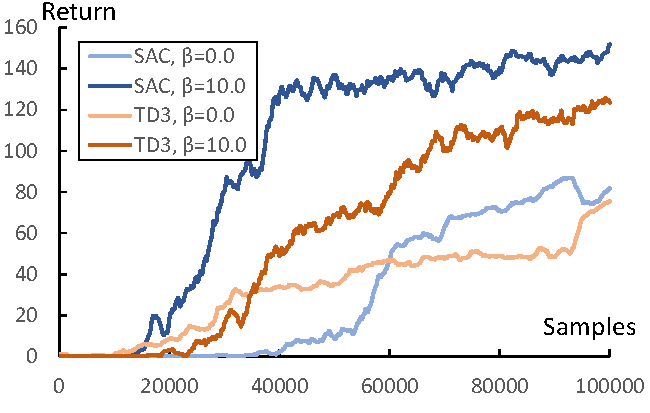
\includegraphics[width=180pt]{figs/SHC.pdf}}
   \subfigure[Deceptive HalfCheetah task]{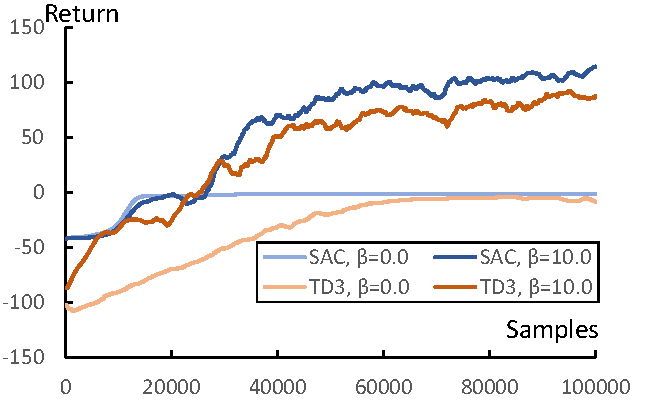
\includegraphics[width=180pt]{figs/DHC.pdf}}
   \caption{Mean return curve for SAC and TD3 on HalfCheetah task.}
   \label{fig:GymHC}
\end{figure}

\begin{figure}[hbt]
   \centering
   \subfigure[Sparse ContinuousMountainCar task]{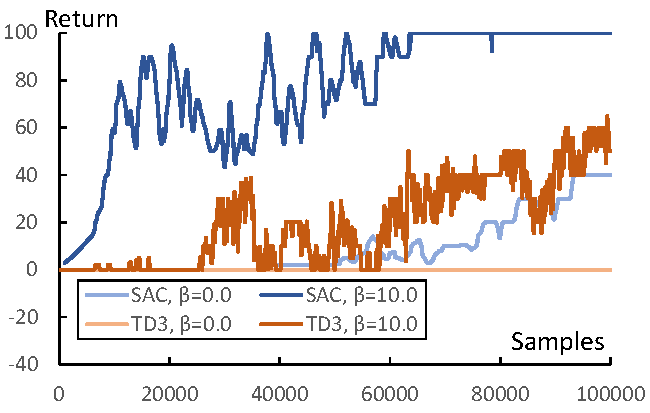
\includegraphics[width=180pt]{figs/SCMC.pdf}}
   \subfigure[Deceptive ContinuousMountainCar task]{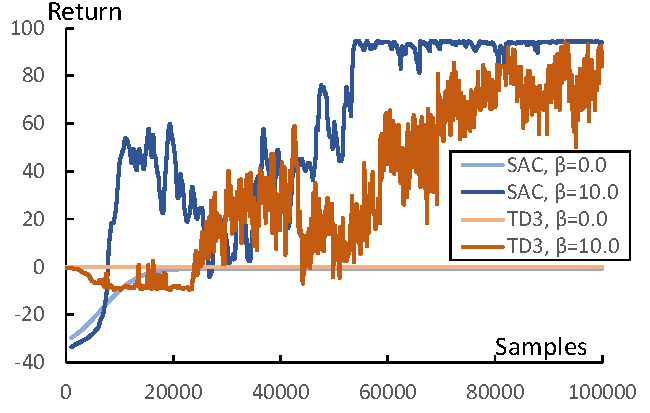
\includegraphics[width=180pt]{figs/DCMC.pdf}}
   \caption{Mean return curve for SAC and TD3 on ContinuousMountainCar task.}
  \label{fig:GymCMC} 
\end{figure}

It can be seen from the experimental results in Fig \ref{fig:GymCMC} and Fig \ref{fig:GymHC} that, in all tasks, the task using the LiFE bonus setting can be effective. In the case of $\beta = 10$, the agent can learn to reach the goal and continuously optimize the strategy. In the case of $\beta = 0$, the agent needs more samples to reach the goal or converges to the suboptimal strategy and stops in place.

In addition, we also found that the performance of the SAC algorithm on sparse and deceptive tasks is better than TD3. We consider that this is because the SAC algorithm uses a maximum entropy method that automatically adjusts parameters. The $\sigma$ of the Gaussian actor is relatively high at the beginning of training, resulting in a high exploration level and increasing the probability of visiting the goal. The average entropy of the actor will decrease with the training progress and converge to the optimal policy. TD3 relies on fixed action noise on the actor for exploration, and the exploration ability is limited. However, the maximum entropy strategy is a non-directional exploration method, so deep exploration cannot be achieved. The results indicate that combining deep exploration strategies such as LiFE bonus will achieve higher sample efficiency.
\section{Conclusion}
This article summarizes the reasons that lead to difficulties in exploring sparse/deceptive tasks as "zero rewards" and "action penalty" and indicates how these factors affect reinforcement learning algorithms. We propose the LiFE method: use the input of the last fully connected layer of the neural network as the feature representation to calculate the feature matrix for measuring uncertainty, and calculate the UCB bonus for exploration. 

We designed a low-dimensional continuous action task "swim" to measure the exploration ability of the proposed method. Experimental results show that our method has the ability to explore deeply under different task configurations. We finally tested the modified version of the Gym task using SAC and TD3 as baseline algorithms, and the results show that our method can solve continuous control tasks under sparse/deceptive rewards.

\bibliography{reference}
\bibliographystyle{bibstyle}



\end{document}